%!TEX root = ../../super_main.tex

\section{Measurement Redundancy}
\label{sec:measurement_redundancy}

By the design of our temporal structure of measurement (see \secref{sec:temporal_properties_of_snapshots}), we wanted to provide the customer with a uniform dataset, by having the temporal structure of all sensors to be the same. We thought that a uniform structure would be more convenient for the customer, even though different sensors are of varying nature as discussed in \secref{sec:deriving_the_context_from_sensors}. However, after enforcing this temporal structure on all our sensors, we, as expected, found that there were a lot of data redundancy. An example of this is specifying a campaign to gather Wi-Fi data with a relatively high frequency, the amount of data increased significantly, because it contained information about all access points around the device. This combined with being located at the university, where the density in access points is rather high, we found that enforcing the temporal structure on these type of sensors is more severe than we first assumed. One should consider only gathering a single measurement for on-demand sensors such as location and Wi-Fi instead of treating them as the other sensors. This is illustrated in \figref{fig:new_snapshot}, where the blue measurements for the Wi-Fi sensor could be obmitted. This would decrease the data redundancy and still describe the context. However, this would decrease the level of detail the snapshots have in respect to these sensors, and also make the structure of the snapshots less uniform. Nevertheless, it would decrease the consumption of various resources such as memory, disk, battery and internet bandwidth, and could therefore be a significant improvement to the system. 

\begin{figure}[!htbp]
    \centering
    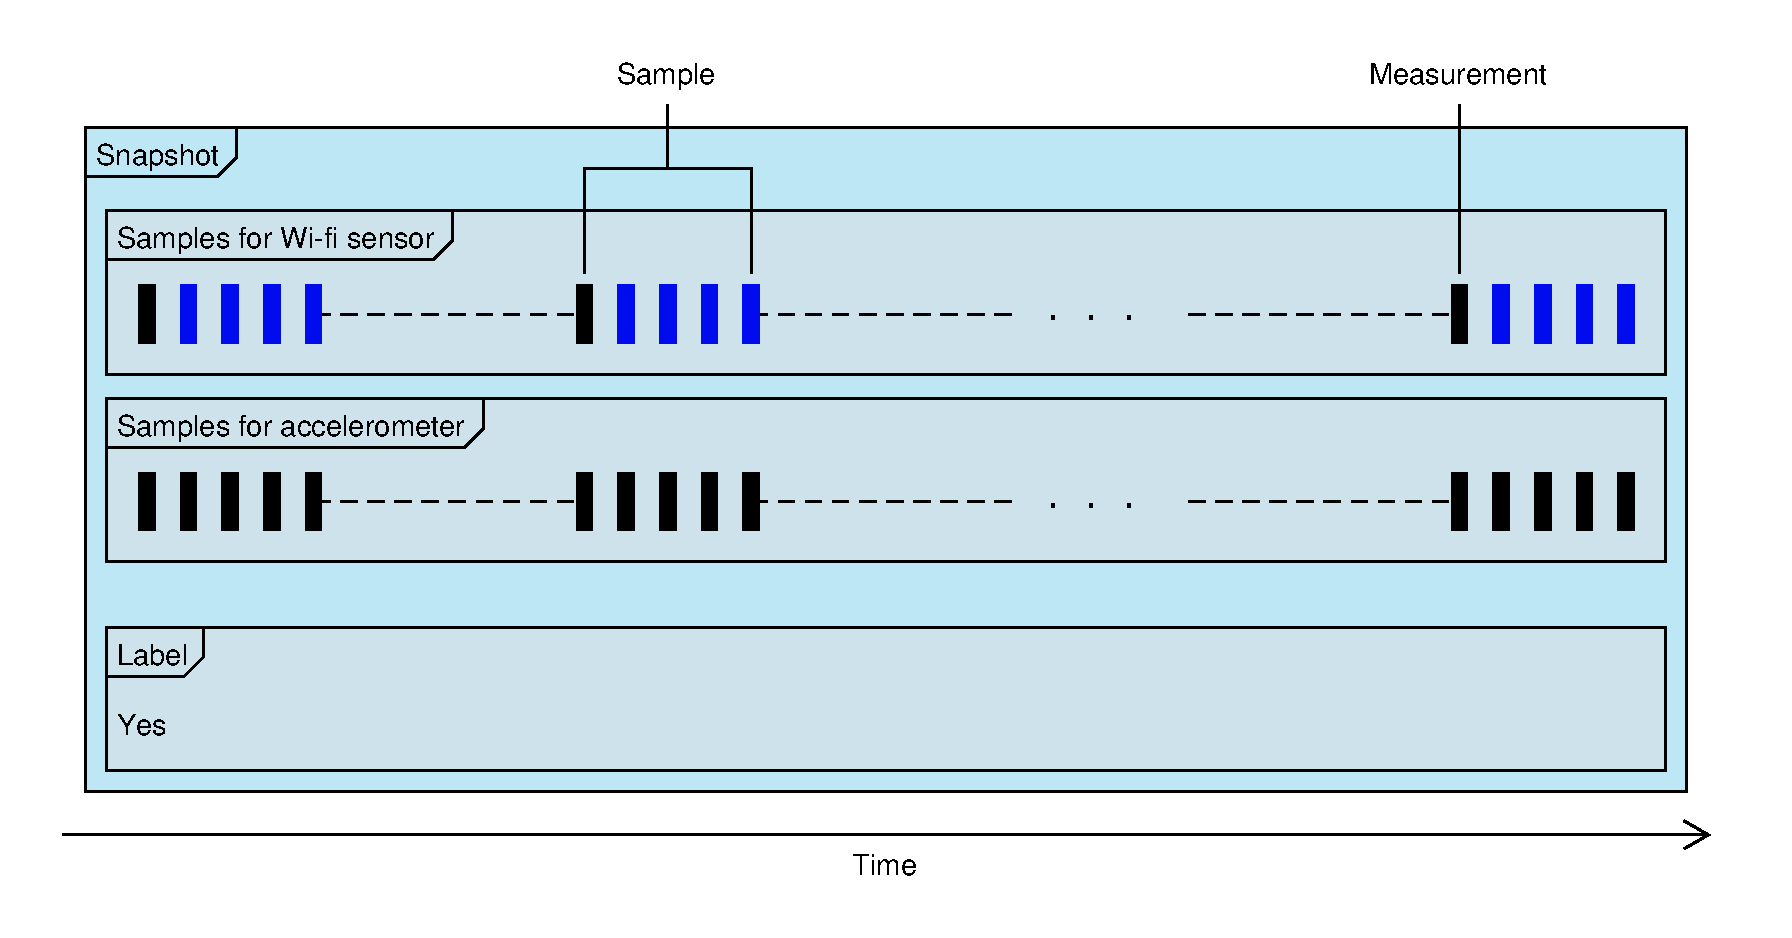
\includegraphics[width=\textwidth]{graphic/reflection/snapshot}
    \caption{Illustration of measurements which could be obmitted.}
    \label{fig:new_snapshot}
\end{figure}
\FloatBarrier